\documentclass[conference]{IEEEtran}

\usepackage[nolist]{acronym}
\usepackage[backend=bibtex]{biblatex}
\usepackage{graphicx}

\addbibresource{vision-transformer.bib}

\hyphenation{op-tical net-works semi-conduc-tor}


\begin{document}

  \title{Exploring artefacts of \acl{vit} feature maps}

  \author{\IEEEauthorblockN{Florian Weidner}
    \IEEEauthorblockA{Philipps-University Marburg, Germany\\
      Department of Mathematics and Computer Science, Deep Learning Group\\
      February 09, 2025\\
  }}

  \maketitle
  \begin{abstract}
  The abstract goes here.
  \end{abstract}

  \begin{IEEEkeywords}
    \acp{vit}
  \end{IEEEkeywords}

  \IEEEpeerreviewmaketitle

  \section{Introduction}

  Transformers \cite{transformer2017} using multi-head self-attention mechanisms have become the model of choice for \ac{nlp} tasks. The approach to pre-train the model on large text data and then finetune on a smaller task-specific dataset has been very successful. The self-attention mechanism allows the modal to learn global contexts and long-range dependencies. With the efficiency and scalability of transformers, it became possible to train very large models with many parametes. \cite{transformer2017} \cite{visiontransformers2021} \cite{vit-state-challenges}

  \acfp{vit}, introduced by \cite{visiontransformers2021}, that use the transformer architecture for computer vision tasks, also became the state of the art architecture, achieving high prediction performance. They can learn rich visual representaions of images. 


  \section{Vision Transformers}

  % \begin{figure}
  %   \centering
  %   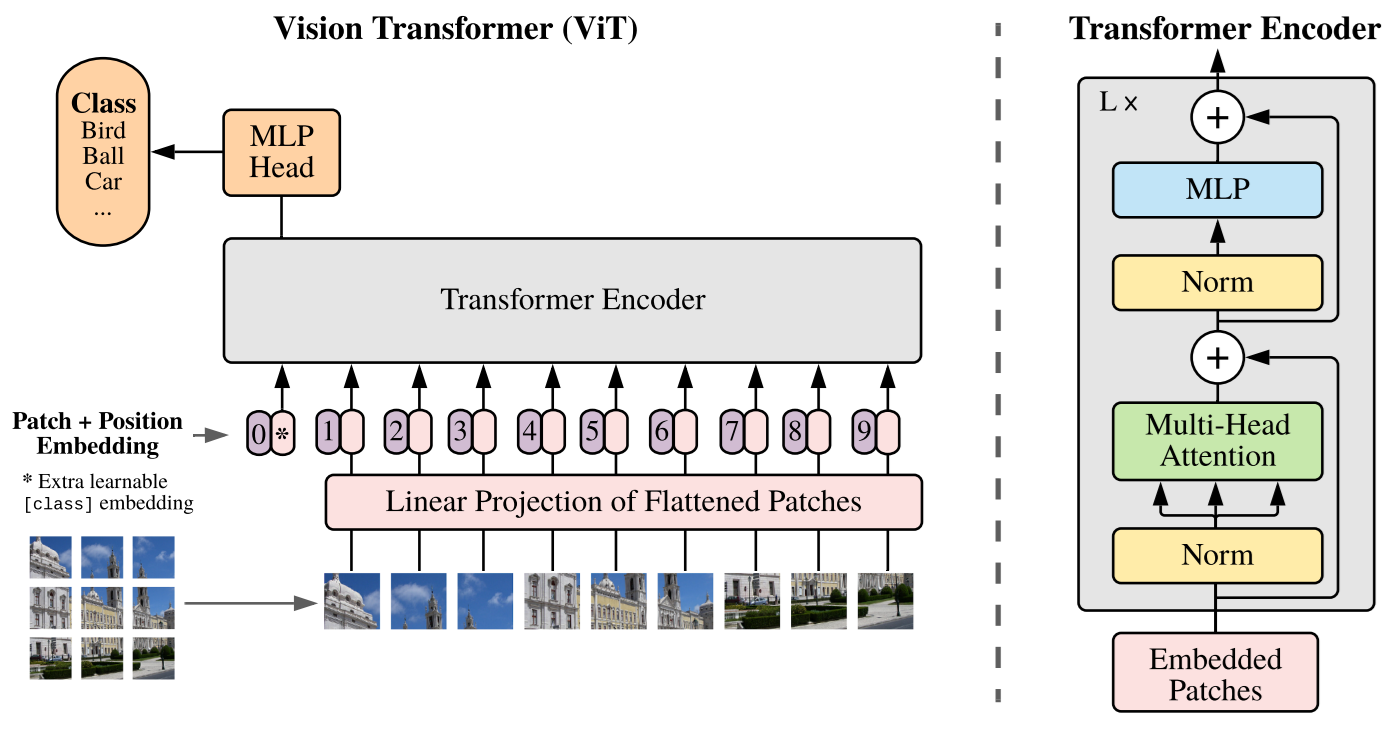
\includegraphics[width=0.5\textwidth]{figures/vit-architecture.png}
  %   \caption{Overview of a \ac{vit} architecture. Image obtained from \cite{visiontransformers2021}}
  %   \label{fig:vit-architecture}
  % \end{figure}

  The Transformer architecture is a neural network model architecture, created primarily for sequence-to-sequence tasks in \ac{nlp}. 
  \begin{quote}
    "The key feature of transformers is the self-attention mechanism, which helps a model learn the global contexts and enables the model to acquire the long-range dependencies." \cite{vit-state-challenges}
  \end{quote}
  It consists of an encoder, which makes the input sequence into a continuos representation and a decoder, which then generates the output sequence. The encoder is built up of n identical layers, containing following components:
  \begin{itemize}
    \item multi-head self-attention mechanism: captures relationships between all tokens in the input, regardless of their distance
    \item feed-forward network: simple two-layer MLP network with ReLU activation which is applied to each token separately
    \item add \& norm layers using residual connections and layer normalization to stabilize the training
  \end{itemize}
  The result outcome of the encoder is a enriched sequence representation, which is then used by the decoder to generate the output sequence. The decoder also consits of n identical layers with:
  \begin{itemize}
    \item masked multi-head self-attention mechanism: ensures a causal generation, by preventing that tokens have impact to future tokens
    \item encoder-decoder attention mechanism: focuses on the relevant parts of the encoder's output
    \item feed-forward network: similar to the encoder
    \item add \& norm layer:ssimilar to the encoder
  \end{itemize}
  The input text is embedded and combined with a positional encoding to provide token order information. Because several attention layers can run in parallel, the architecture is significantly more parappelizable than \ac{rnn} or \ac{cnn} architectures, which makes it very efficient for modern hardware accelerators. That allows the Transformer to scale to very large models and datasets. \cite{transformer2017}

  \citeauthor{visiontransformers2021} introduced the idea of using the stated transformer architecture for computer vision. A lot of research tried to combine self-attention mechanisms with \ac{cnn} architectures, not achieving a effectively scalable method for modern hardware accelerators. \cite{visiontransformers2021} proposed to apply a standard Transformer directly to images, that are split into fixed-size patches. Each patch is flattened into a vector and passed through a linear projection layer to form an embedding as input for the Transformer. These embeddings are used as tokens in a \ac{nlp} scenario. Positional embeddings are added to retain spatial information since they process images as sequences, unlike \acp{cnn} which inherently capture spatial hierarchies. For classification tasks, an extra learnable [class] embeding is added in front of the embedded input. At the output of the encoder, the final representation of this token is used for classification. Instead of using encoder and decoder like in \ac{nlp} tasks, acp{vit} only uses the encoder since the goal is to find a better representation but an autoregressive prediciton. Additional Layer Normalization is used before the multi-head attention laver. \cite{vit-state-challenges} In figure \ref{fig:vit-architecture} you can see the architecture of a \ac{vit} including the split image patches, their embeddings combined with positional embeddings the encoder and the class embedding used for the classificaion prediction.
  \acp{vit} have much less image-specific inductive bias than \acp{cnn}, because other than \acp{cnn}, with the global self-attention mechanism spatial relationships needs to learned from scratch, but long-range dependencies across the entire image can be captured. As Transformers, \acp{vit} are normally pre-trained on large datasets and then fine-tuned to more specific tasks. After pre-training, the prediction head is removed and a zero-initialized feedforeward layer, where the size is the number of classes, is added.

  Like Transformers, \acp{vit} are also very parallelizable, which makes them very efficient. But \cite{visiontransformers2021} found out that without large-scale pre-training, \acp{vit} often underperform. So \acp{vit} requires sidnificant computational resources. But when pre-trained on large datasets, \acp{vit} outperforms \acp{cnn} on image classification tasks. The architecture performs well for transfer learning, where the pre-trained model can be fine-tuned already with limited labeled data \cite{visiontransformers2021}.  \cite{visiontransformers2021} stated that further scaling of \acp{vit} would likely lead to improved performance. Also self-supervised pre-training, where no labeled data is needed, can be improved. They found out that with mimicking the masked language modeling task used in BERT, the model performs still better than \acp{cnn} but a bit worse that with supervised pre-training of a \ac{vit}. By now different architectures and training-tricks of \acp{vit} have been proposed to further improve \acp{vit} including self-supervised learning. The architectur also got adapted for image recognition, object detection, image segmentation, pose estimation, and 3D reconstruction tasks. \cite{vit-state-challenges}

  The classical \ac{vit} architecture has been adopted and improved by many others. One approach is to include \ac{cnn} structures, which bring locality through the convolution kernels, into \acp{vit} to improve the data efficiency. DeiT \cite{deit} for example uses a \ac{cnn} as a teacher to train a \ac{vit}. It utilizes knowledge distillation of the \ac{cnn} to add the inductive bias to a vision transformer. It allows to train a \ac{vit} without the need of large-scale pre-training the model. \cite{vit-state-challenges} Another approach is to diversify the features of \acp{vit}. DeepVit \cite{deepvit} found out that the attention collapses in deeper layers, wich leads to lower performance. By adding a learnable transformation matrix after the attention layer, the model is stimulated to generate new attention maps also in the deeper layer, increasing the performance. \cite{vit-state-challenges} Also the heavy computation costs are reseached. Many also try to improve the self-supervised learning, that the pre-training with the need of large datasets can be simplified. \cite{vit-state-challenges} The following summerized paper, identifies and addresses artifacts in attention maps of supervised and self-supervised \ac{vit} networks.
  
  In the following chapter the concepts of different \ac{vit} architectures are introduced. These models are used in the paper \cite{registers} that will be summerized afterwards.

  \subsection{\mbox{DINO} and \mbox{DINOv2}}
  \cite{dino} \cite{dinov2}
  \mbox{DINO} is a self-supervised learning framework using a student-teacher network. The teacher is dynamically built from past iterations of the student network. It uses self-destillation with no labels. For each image, two high-resolution global views and several low-resolution local views are generated. The teacher only processes the global views using an Exponential Moving Average of the student's weights. The student processes global and local views and the cross-entropy loss is used to calculate the similarity between the student and teacher. It also uses mechanisms to avoid trivial solutions. \cite{dino} It is shown that the the attention maps contain explicit information about the semantic layout of an image. \cite{registers}

  \mbox{DINOv2} further improves the idea of \mbox{DINO}, enhancing scalable, efficiency and genalization of self-supervised learning in computer vision. Following techniques are used to improve the model:
  \begin{itemize}
    \item  using an automatic pipeline to build a dedicated, diverse, and curated image dataset
    \item  using bigger \ac{vit} model with one bilion parameters
    \item distilling the model into a series of smaller models \cite{dinov2}
  \end{itemize}
  The improvments enable dense prediciton tasks. On the other hand, artifacts in the attention maps of \mbox{DINOv2} are observed. \cite{registers}

  \subsection{OpenCLIP}
  \mbox{OpenCLIP} is a open source implementation of \ac{clip} \cite{clip} from OpenAI, which uses language-image pre-training to enable zero-shot transfer to a wide range of tasks. \ac{clip} tries to predict the caption of an image. It tries to maximize the similarity between correct pairs and minimizing the similarity for incorrect paris. The pre-trained model, that outputs text from an input image, can be used to extract information from the output text for various specific tasks. The models are competetive with compared supervised models that are specifically trained for the task. \cite{clip}
  \mbox{OpenCLIP} has trained several models of different sizes with different data sources. \cite{open-clip} 

  \subsection{\mbox{DeiT-III}}
  \mbox{DeiT-III} focuses on supervised training of \acp{vit}, trying to create a new baseline for supervised \ac{vit} models. A new data augementation approach, inspired by self-supervised learning techniques is used before training. Also they use Simple Random Cropping insted of Random Resize Cropping. The image resolution has been lowered. With a change from 224 × 224 to 126 x126, 70\% fewer tokens are used. It turned out to prevent overfitting for the larger models and achieves better performance. Additionally they adopted the binary cross entropy loss, which improved the training of large \acp{vit}. \cite{deit3}



  \subsection{LOST}
  \label{chapter:lost}
  \mbox{LOST} is a self-supervised object discovery algorithm, that can be used to detect objects in an image without the need of any labled data. To find an object in an image it uses a \ac{vit} model like \mbox{DINO} and feeds the image through the \ac{vit}. It is assumed that every image has at least one object. Instead of looking at the class token for classificaion results, the attention maps of the last layer are used to compute similarites between differnt patches. The patch with the smallest number of positive correlation with other pathces is used as the \textit{seed}. They state that is likely hit an object because
  \begin{quote}
    "patches within objects correlate more with each other than with background patches and vice versa, and ... an individual object covers less area than the background. Consequently, a patch with little correlation in the image has higher chances to belong to an object." \cite{lost}
  \end{quote}
  After selecting the \textit{seed}, additional patches correlating with the seed are searched, because they are also likely to belong to the same object. After that a bounding box is calculated by comparing the seed features with all the image features. The fact that the method detects objects on a single image, without the need of exploring the image collection, makes it very scalable. After that a class-agnostic detection model is trained with the generated bounding boxes. Here also more objects in one image can be detectd. It also turns out the trained model is better than just \mbox{LOST}. This method provides pseudo-boxes without a category of the object. To also detect a semantic category in a self-supervised way, the usage of K-means clustering is presented. The detected objects are cropped and resized and then fed throug a \mbox{DINO} pre-trained transformer. The class tokens is then extracted and than clustered with the K-means algorithm. That gives pseudo-labels that are matched with the ground truth labels at evaluation time using the Hungarian algorithm. \cite{lost}



  \section{Vision Transformers need registers: A summary}

  In this chapter we summerize the paper \cite{registers}. The paper discoverd artifacts and proposes to use additional register tokens for \acp{vit} to remove these artifacts.

  \subsection{Artifacts in Vision Transformers}

  % \begin{figure}
  %   \centering
  %   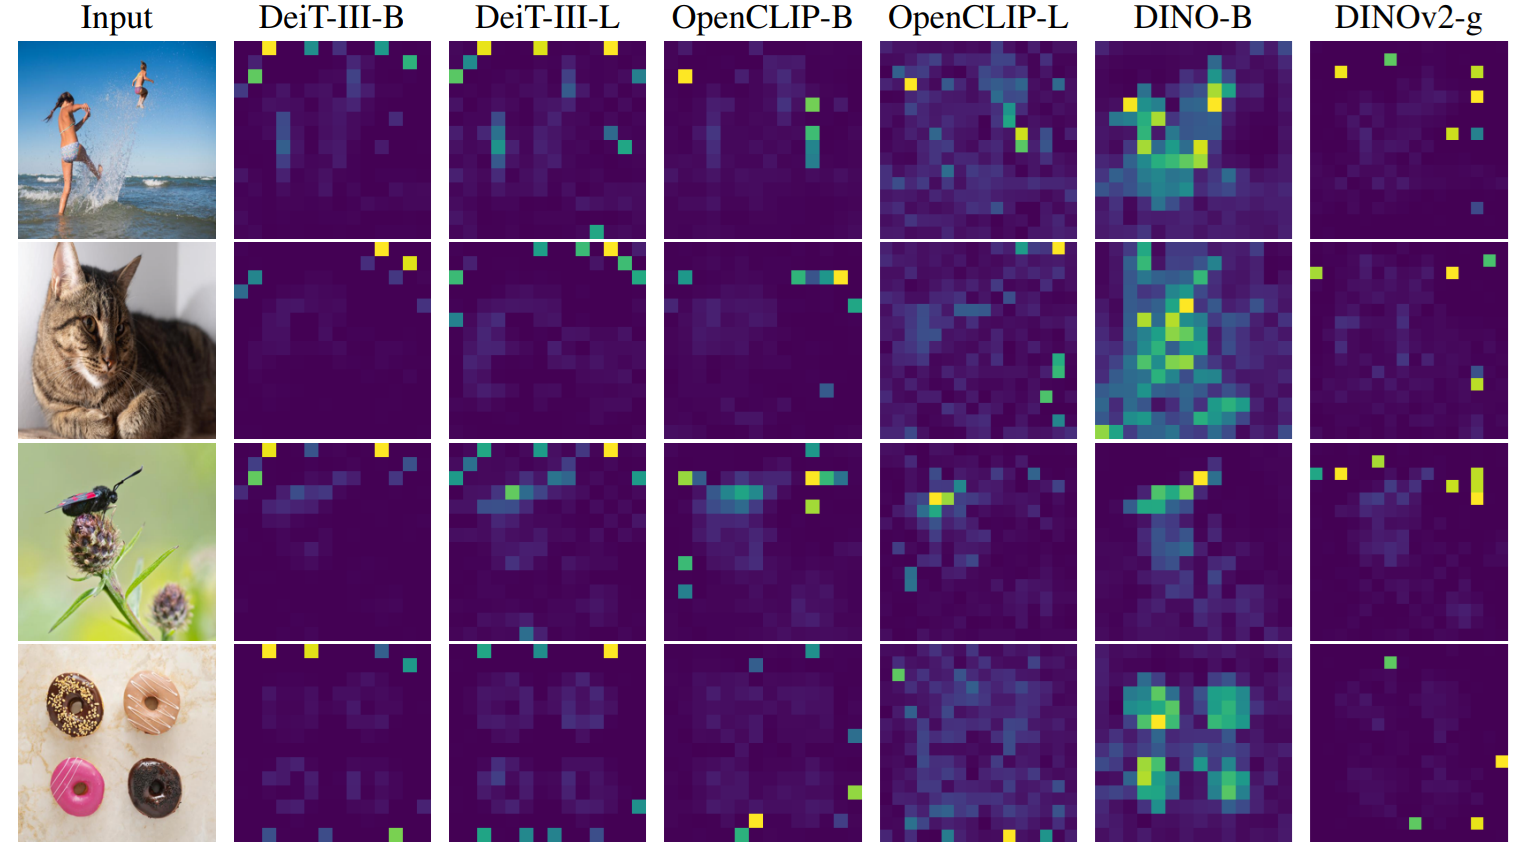
\includegraphics[width=0.5\textwidth]{figures/vits-artifacts.png}
  %   \caption{Illustration of artifacts observed in the attention maps of modern vision transformers. Image obtained from \cite{registers}}
  %   \label{fig:artifacts-observations}
  % \end{figure}


  After introducing to \acp{vit} like we did in this paper, the models they found the artifacts are introduced. The \mbox{DINO} algorithm is a self-supervised learning method, that uses two \acp{vit}. A student network is predicting the output of a teacher network, to learn rich representaions of visual data without the need of manual annotations. \cite{dino} \mbox{DINO} is shown to produce models, that contain semantically consistent information in the last attention layer. Object discovery algorihtms like \mbox{LOST} \cite{lost}, built on top of \mbox{DINO}, are using these attention maps, that often contains semantically interpretable information, used to detect objects without supervision. \mbox{DINOv2} \cite{dinov2} is a improved followup focusing on dense predition tasks, which are tasks, where detailed outputs are required to provide fine-grained localized informations, like semantic segementation or depth estimation. Despite good performance on these dense tasks, the authors observed that \mbox{DINOv2} is incompatible with \mbox{LOST} \cite{registers}. The different behaviour of \mbox{DINO} and \mbox{DINOv2} can be observed in the artifacts in the last attention maps. In figure \ref{fig:artifacts-observations} you can see the different models and their artifacts on the last attention layer.
  While \mbox{DINO} shows no peak outlier values focusing the main object in the image, \mbox{DINOv2} shows a lot of artifacts on the background of the images. This qualitatively observation can be also made for the label-supervised model \mbox{DeiT-III} and the text-supervised model \mbox{OpenCLIP}. Shown in figure \ref{fig:artifacts-observations}, you can observe similar artifacts in the background.
  To explain why and where the artifacts of \acp{vit} in attention maps appear, the paper focuses on \mbox{DINOv2}. 

  Artifact patches show higher norm of their token embedding at the output of the model than other patches. In figure \ref{fig:artifacts-norm} you can see the distribution of the local feature norms over a small dataset. While for \mbox{DINO}, the norm stays under 100 for all patches, \mbox{DINOv2} shows a lot of patches with a norm higher than 150. This cutoff value can vary across different models. They define artifacts as
  \begin{quote}
    "tokens with norm higher than 150 will be considered as “high-norm” tokens" \cite{registers}
  \end{quote}

  The authors found different conditions, when the artifacts appear in the training process of \mbox{DINOv2}. Figure \ref{fig:artifacts-layer} shows the following conditions:
  \begin{itemize}
    \item artifacts start appearing around layer 15 to 40.
    \item artifacts start appearing after on thrid of training.
    \item artifacts only appear in the three largest model versions
  \end{itemize}

  % \begin{figure}
  %   \centering
  %   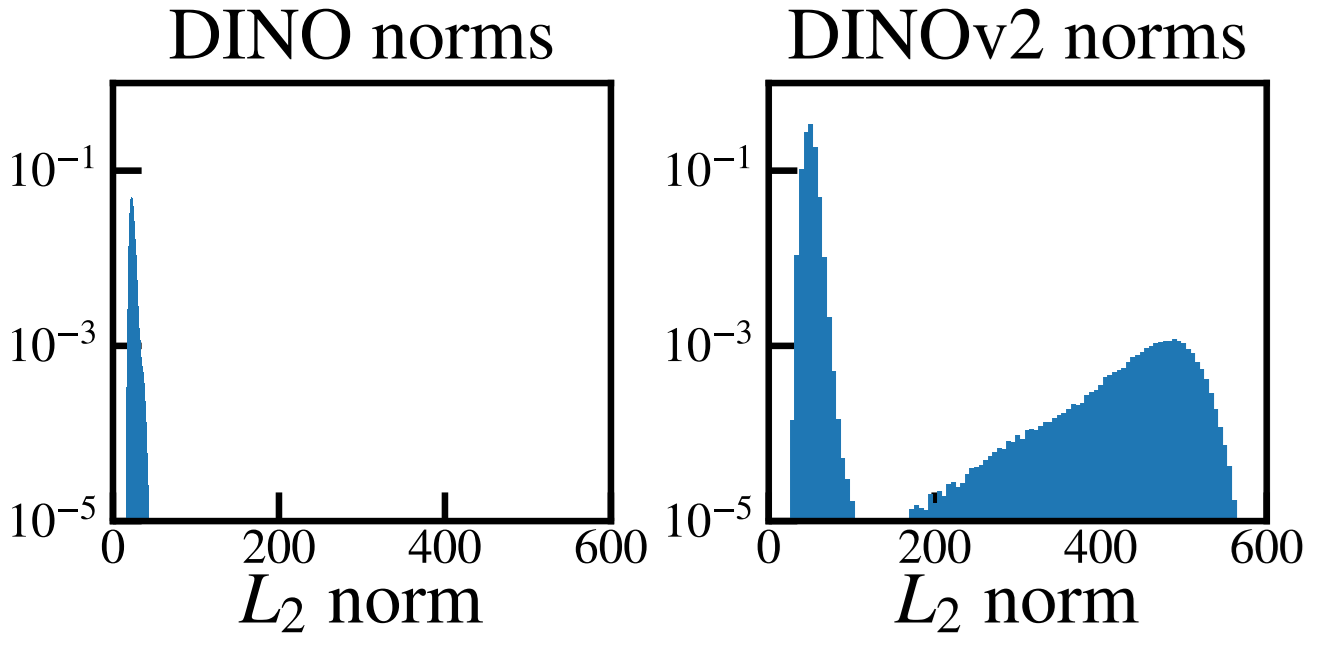
\includegraphics[width=0.3\textwidth]{figures/artifact-norm.png}
  %   \caption{Comparison of local feature norms for \mbox{DINO} ViT-B/16 and \mbox{DINOv2}. Image obtained from \cite{registers}}
  %   \label{fig:artifacts-norm}
  % \end{figure}
  % \begin{figure}
  %   \centering
  %   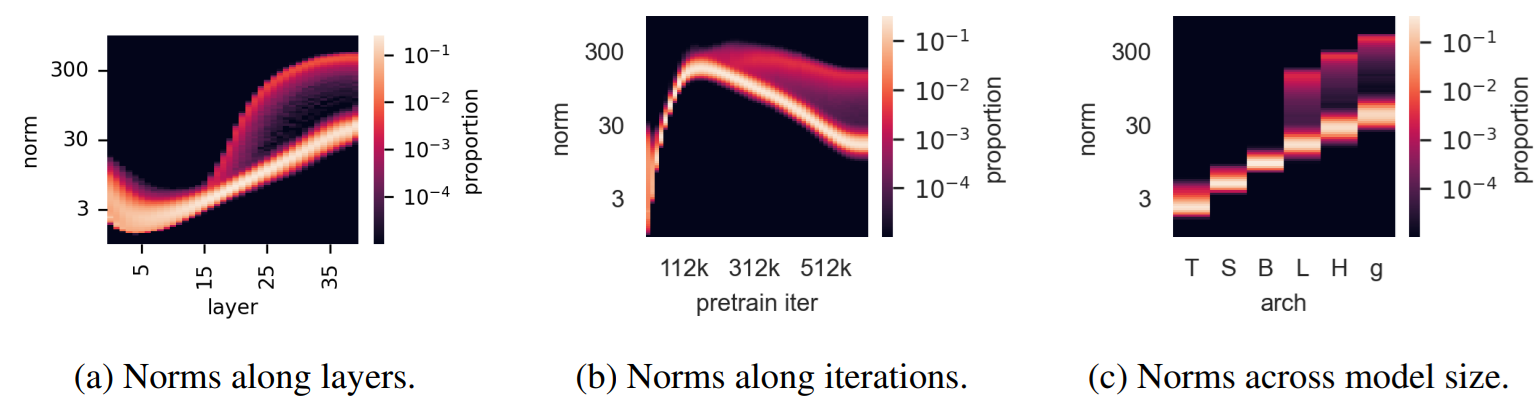
\includegraphics[width=0.5\textwidth]{figures/artifact-layers.png}
  %   \caption{Illustration of several properties of outlier tokens in the 40-layer \mbox{DINOv2} ViT-g model. Image obtained from \cite{registers}}
  %   \label{fig:artifacts-layer}
  % \end{figure}

  Another discovery is that the high-norm tokens appear where patch information is redundant. The authors tested the cosine similarity between high-norm tokens and their four neighbors, directly after the image is emebdded. They observed, that the high norm patches appear where their cosine similarity to the neighbors is high. Compared to the observations, that shows that artifacts appear mostly in the background of images, high-norm pathes seem to have redundant information, that the model can ignore, to achive similar scores at the output.

  To further understand the outlier tokens, two linear models were trained, to check the embeddings for different information. Both models were trained on the patch embeddings, the embeddings of the images (see figure \ref{fig:vit-architecture}). The result performance is compared between using high-norm tokens and normal tokens. The first task was position prediction. The model should predict the position of a patch token in the image and measure the accuracy. They observed that high-norm tokens have much lower accuracy than the other tokens and suggested that they contain less information about the position in the image. The second task was pixel reconstruction. The model should predict the pixel value of an image from the patch embeddings and mesaure the accuracy of this model. Also here the high-norm tokens have  lower accuracy than the other tokens. The authors concluded that the high-norm tokens contain less information to reconstruct the image than the others. 
  The authors also found out that the high-norm tokens hold more global information by training a logistic regression model. The model predicts the image class by the patch embedding of a random token. I turned out that the high-norm tokens have a much higher accuracy than the other tokens. This suggests that the high-norm tokens contain more global information about the image than the other tokens. 

  Making these obervations the authors make following hypsthesis:
  \begin{quote}
    "Large, sufficiently trained models learn to recognize redundant tokens, and to use them as places to store, process and retrieve global information." \cite{registers}
  \end{quote}

  \subsection{Registers for Vision Transformers}


  To address the behaviour, the use of registers is proposed. Since the high-norm patches are overtaking local patch information, even they are mostly not important, it possibly decreases the performance on dense prediction tasks. The called registers are additional tokens after the patch embeddings of the images with a learnable value. They work similar to the [class] token, used for classificaion tasks. They are used durning training and inference and they are discarded afterwards. In figure \ref{fig:register-architecture} you can see the register tokens additionally used after the embedding of the image. A complexity analysis show that adding registers increase the FLOPs by up to 6\% for 16 registers. With four registers, that are more commonly used, the increase is below 2\%.

  % \begin{figure}
  %   \centering
  %   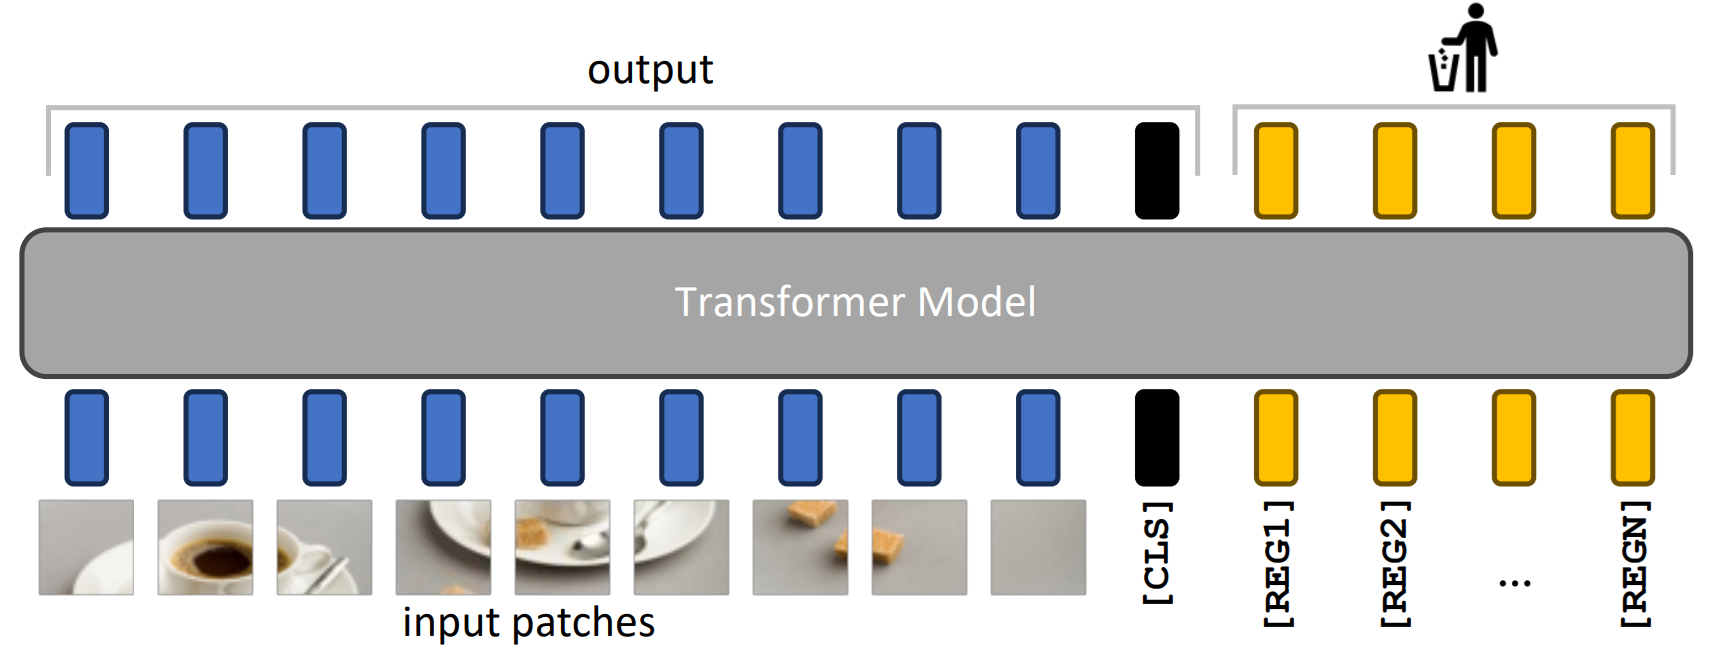
\includegraphics[width=0.5\textwidth]{figures/register-architecture.png}
  %   \caption{Illustration of the proposed remediation and resulting model. Image obtained from \cite{registers}}
  %   \label{fig:register-architecture}
  % \end{figure}

  The idea of adding additional tokens as memory to a transformer model is from \cite{memorytransformer}. The study adds trainable memory to transformer for \ac{nlp} tasks. Many studies before have tried memory augementation in neural networks, to imporve the performance of the models. For Transformers the paper use general purpose [mem] tokens that can be used as placeholders by the model, to store global information or copy also local representaions. They are proposing three different architectures using memory tokens. The first one is just concatenate the tokens to the input, and process them together in one encoder by layers with the same parameters. This is the approach that is adapted for the register tokens of the \ac{vit}. The second architecture of \cite{memorytransformer} is to use a sepereate memory control layer and the third architecture further restricting the processing by first updating the attention of the memory and then update the attention maps of the sequence. The evaluation showed that the basic memory architectur outperforms baseline transformers. The other architectures had not so clear results, sometime increasing, sometimes decreasing performance of baseline transformers.

  \subsection{Evaluation of the proposed architecture}

  In the last part of the paper they validate their architecture by training \acp{vit} with register tokens and compare them  quantitativly and qualitativly to the models without token registers. They are evaluating for \mbox{DeiT-III}, \mbox{OpenCLIP} and \mbox{DINOv2} architectures, therfore including label-supervised, text-supervised and self-supervised learning approaches. In figure \ref{fig:register-result} you can see three example images including attention maps with and without the use of register tokens. Qualitativly, for all three models, the artifacts in the attention maps are gone. They mesaured quantitativly the effect by calculating the norm of the attention maps at the output of the model. In figure \ref{fig:register-norm-result} you can see the distribution of the output norms for the three models. For all three models, training it with register tokens removes high-norm tokens, that were present without the token registers. Instead the attention maps of the register tokens have  higher norm than the patch and the class tokens. The register tokens are adapting the behaviour of the outlier patches of the model without registers. Visualizations are also showing that the attention maps of the register tokens look similar to the attention maps of the class tokens, all showing a larger support area. The attention maps of the patch tokens are more localized. Since the class token carries global informations, it suggests that the register tokens are also used to store global information. 
  Comparing the performance of the models with and without register tokens, linear probing on ImageNet classification, ADE20k Segmentation, and NYUd monocular depth estimation datasets was used. The results show no lose in performance, when additoinally using register tokens. Also for zero-shot classification on ImageNet with \mbox{OpenCLIP}, the performance is not affected by using register tokens. They also found out that one register is enough to remove the high-norm tokens in the attention maps. For \mbox{DINOv2} and \mbox{DeiT-III}, adding register tokens significantly improves the discovery performance and for \mbox{OpenCLIP}, the performance is slighty worse with registers. The authors concluded that their proposal isolates the behaviour of the model using memory for global information. It was shown that \acp{vit} naturally using patches to store global information. With creating registers exactly for that purpose, collateral side-effects, like bad performance of \mbox{LOST} with \mbox{DINOv2} can be avoided.

  % \begin{figure}
  %   \centering
  %   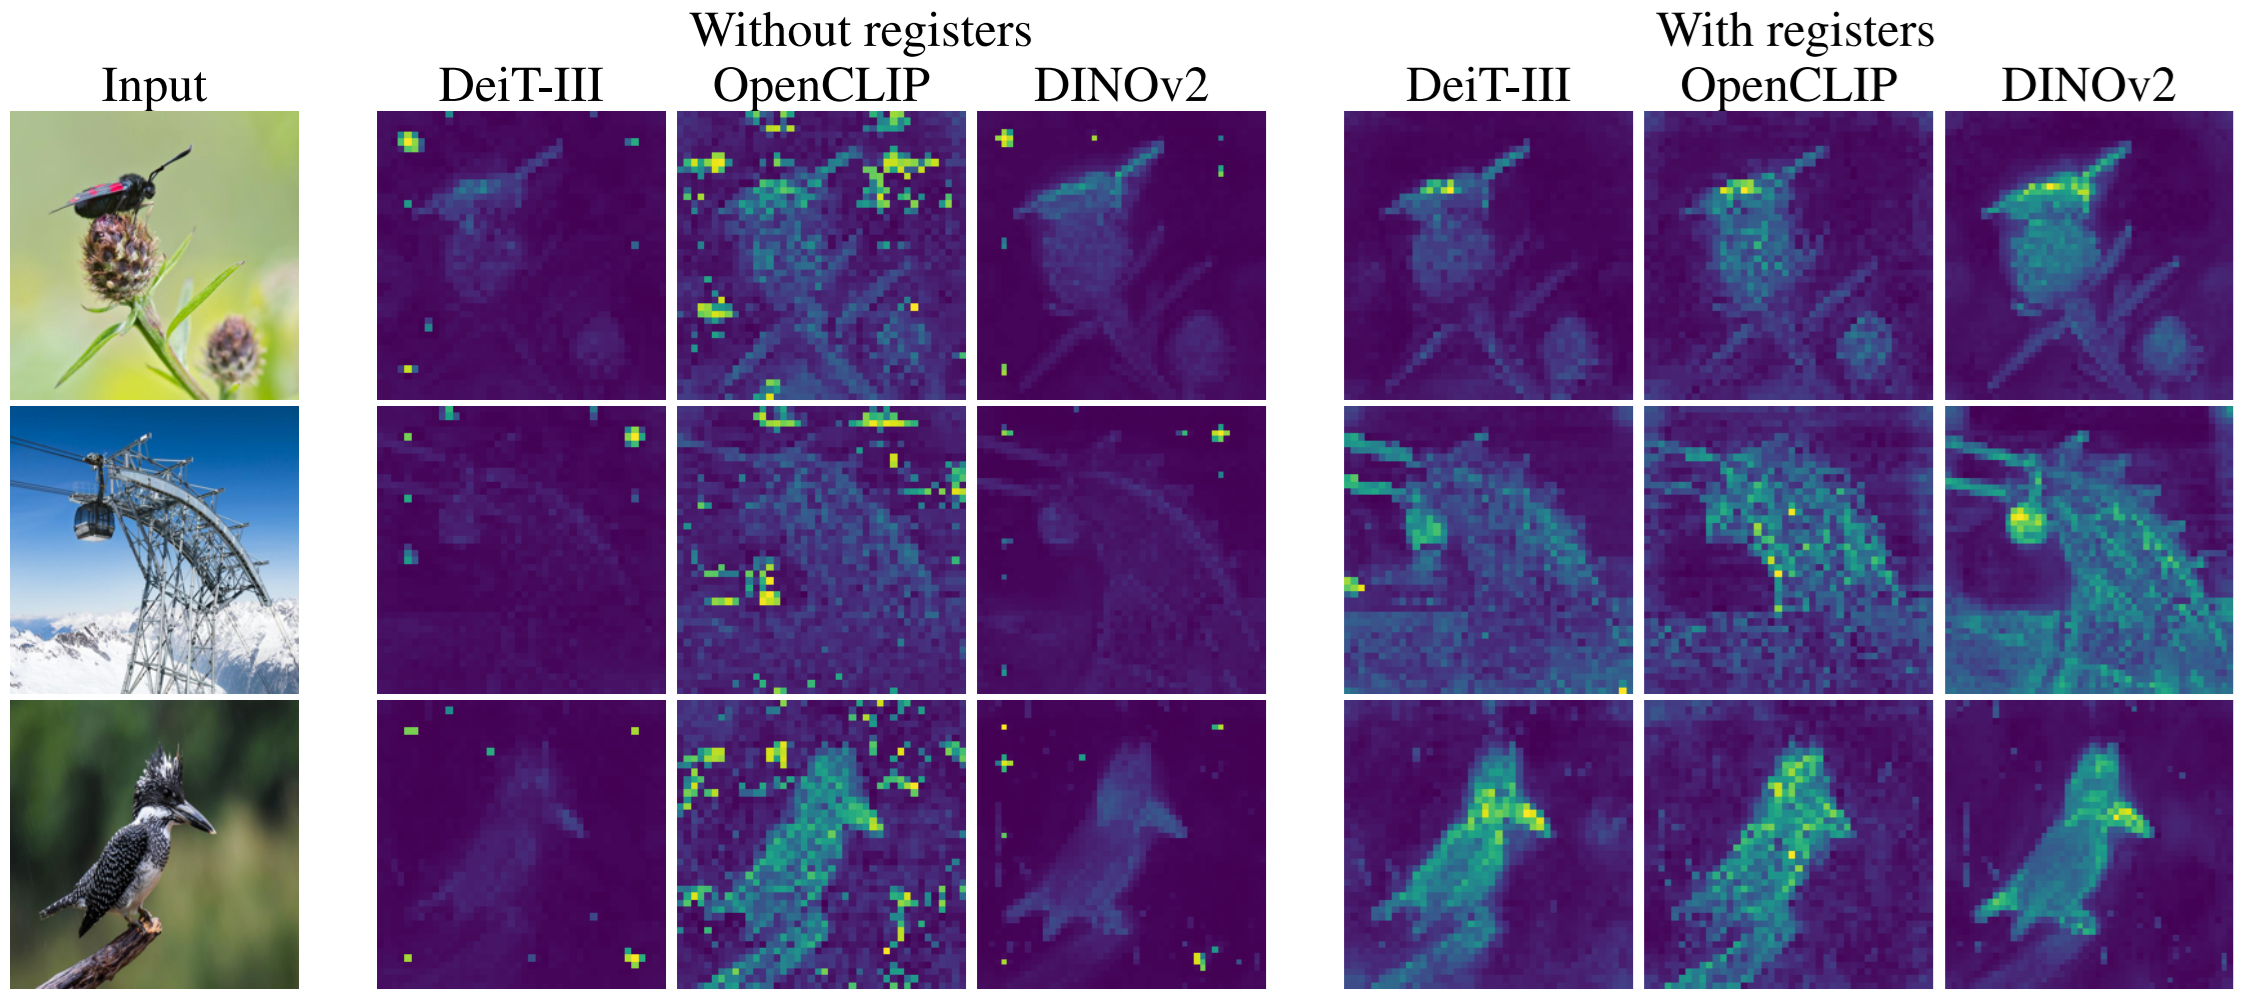
\includegraphics[width=0.5\textwidth]{figures/register-result.png}
  %   \caption{Three examples of attention maps with and without register tokens. Image obtained from \cite{registers}}
  %   \label{fig:register-result}
  % \end{figure}

  % \begin{figure}
  %   \centering
  %   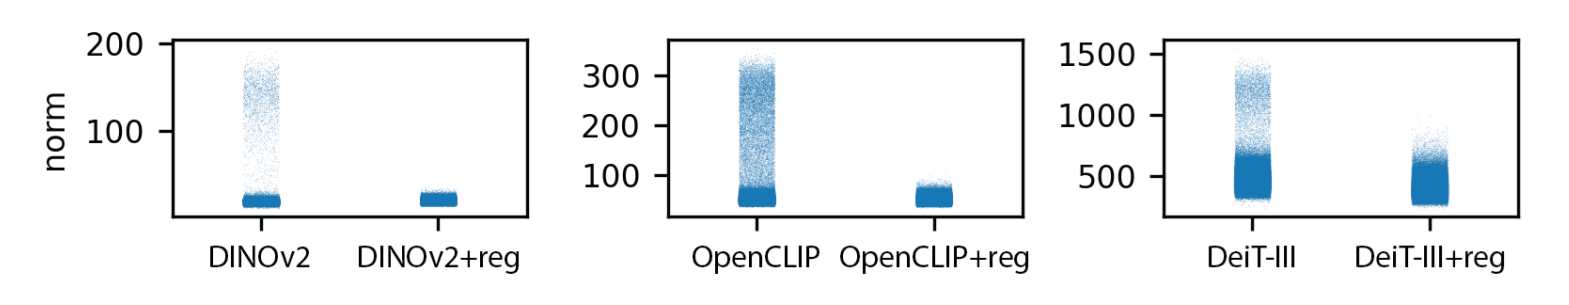
\includegraphics[width=0.5\textwidth]{figures/register-norm-result.png}
  %   \caption{: Effect of register tokens on the distribution of output norms. Image obtained from \cite{registers}}
  %   \label{fig:register-norm-result}
  % \end{figure}


  \section{Comparison to other papers with performance improvements of \ac{vit}s}

  \subsection{\cite{mamba-needs-registers} applies the idea of registers to a \ac{ssm}}
  The authors applied the use of register tokens to the Vision Mamba model, after also discovering outlier tokens in the background, achieving higher performance than without registers. 
  
  Vision Mamba \cite{vision-mamba} is a model architecture using bidirectional \acfp{ssm}. The VIM Blocks, that are inspired by \ac{ssm} can maintain long-range dependencies in the model, similar like the attention mechanism for \acp{vit}. Otherwise, it uses a feedforeward network, positonal encoding and normalization. Images are also decomposed into patches and then used as input to the Vision Mamba encoder. The big advantage compared to the quadratic complexity of self-attention mechanism is that its computational complexity is only linear. Therefore the training process and the memory usage is way lower than using \acp{vit} and \acp{cnn}. The architectur outperforms \acp{vit} like DeiT \cite{deit} on some tasks, showing the potential of using \ac{ssm} in computer vision. \cite{vision-mamba} \cite{mamba-needs-registers}
  
  The authors found the same artifacts in the feature maps of Vision Mamba than \citeauthor{registers} found artifacts in the attention maps of various \acp{vit}. They even exists considerably more severe in the Vision Mamba, starting already in small models sizes. In figure \ref{fig:mamba-artifacts} you can see the artifacts, which are spread all over the image, but also mainly appearing in background regions of the images. The feature maps of the Vision Mamba, that are used for the analysis, are the $\ell_2$ distances between the global and local outputs. The artifacts appear to have a high normalization. Similar graphes like figure \ref{fig:artifacts-norm} are presented. It is also shown that the artifacts contain global information. Building upon the architecture from \cite{registers} using register tokens, they insert the tokens evenly between the token sequence of the image. Since the tokens are not agnostic to their position in the Vision Mamba, having the registers near the whole sequence of input tokens. Another difference is that they concatenate the register tokens at the end, to use them for the final prediction. Doing that, they observed significant improvements. They also observed that the different registers highlighting different objects or semantic elements within a picture. Since Vision Mamba architecture has no multi-head mechanism like the attention mechanism in \acp{vit}, it offers a lot of information that can be used for interpreting the result of the model. The proposed Mamba® architectur outperforms all prior Mamba variants for image classification and semantic segmentation. \cite{mamba-needs-registers}

  % \begin{figure}
  %   \centering
  %   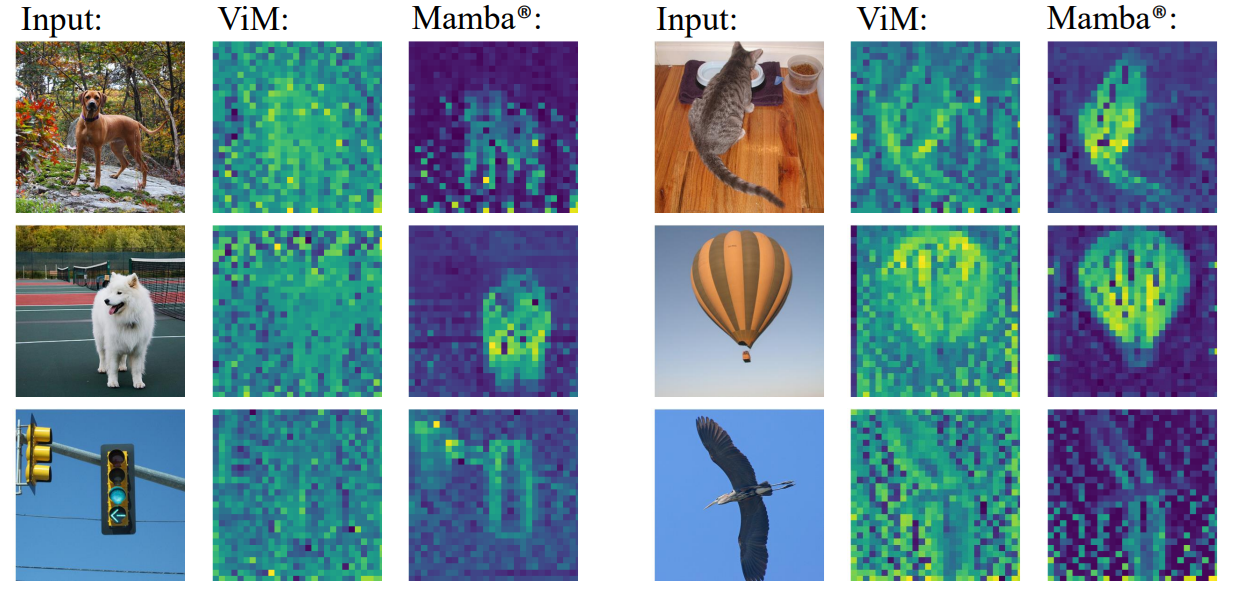
\includegraphics[width=0.5\textwidth]{figures/mamba-artifacts.png}
  %   \caption{Feature maps of vanilla Vision Mamba \cite{vision-mamba} and Mamba® using registers. Image obtained from \cite{mamba-needs-registers}}
  %   \label{fig:mamba-artifacts}
  % \end{figure}

  \subsection{\cite{denoising} uses denoising to remove artifacts}
  The paper also discovers noise artifacts in feature maps of \acp{vit}, including \mbox{DINOv2}, DeIT-III, CLIP and EVA02. They state that the noise hinder feature interpretability and worsens the performance of applying additional methods form the output of \acp{vit} like clustering. The paper focuses on dense recognition tasks, where these artifacts affect the performance of the model, unlike for simple classification. It is hypothesized that positional embeddings play a fole in the appearance of the artefacts. The authors found a correlation between the inclusion of positional embeddings and the emergence of undesirable artifacts in ViT outputs. With the maximal information coefficient, the dependency between grid features and their normalized patch coordinates are measured. The outputs of the original \ac{vit} show a higher spatial correlation than the denoised features (denoised by their solution explained later).
  
  Comparing the \ac{vit} findings from \cite{registers}, artifacts are also observed in small or base \acp{vit} that cannot be easily identified by their high norm values. Also weak artifacts are found in \mbox{DINOv2} using registers. The artifacts are shown in all layers, even using only zeros as input. Shallower layers show more low-frequency patterns that deeper layers, that show more high-frequency patterns.

  The authors propose an aproach to dennoise the feature maps in two steps, without the need to retrain the models, called \acf{dvt}. The first step is per-image dennoising with neual fields, trying to seperate usefull semantic information from the noisy positional artifacts. The authors propose that a feature map can be factorized in three components.
  \begin{itemize}
    \item The clean semantic feature representaion
    \item The artifacts, that depends on the positional embeddings
    \item A residual interaction term.
  \end{itemize}

  For each image, multiple cropped and transformed versions are used to seperate the artifacts from the clean semantic feature representation. The same objects should have similar features across different transformations and artifacts are tied to position that they remain fixed across different transfomations of the image. With the definitions and the use of coordinate networks, known as neural fields, the artifacts can be seperated from the clean representaions over multible iterations with transformed images, minimizing a regularized reconstruction loss. This method effectively removes artifacts from \acp{vit} but needs a high computational effort.

  The second step of the denoising approach trains a genearlizable lightweight denoiser enabling to denoise images in real-time applications. Also denoising the images individually can lead to feature distribution shifts due to the bias of the single images. The denoised images of the first step are used to create a dataset to train a denoiser network. A single Transformer block is used, that learns to map raw \ac{vit} features to denoised features. Additional learnable positional embeddings are added after the foreward pass, to mitigate the input-independent artifacts. The trained model can now also generalize across samples, mitigating the distribution shifts of the first step. In figure \ref{fig:artifacts-positions} you can see the effect of using \ac{dvt} on several images and models. In all images you can see the artifacts, mostly occuring in the background. Also on the model using registers \cite{registers}, weaker but some artefacts are visible. Especially compared to the by \ac{dvt} denoised image. On all denoised images, the artifacts are nearly completely removed. The feature maps of the denoised images show a much clearer and more interpretable objects. Also the performance improvements are visualized. \cite{denoising}

  The authors also stated that artifacts appear in all following task objectives that they evaluated. Here are the results of the evaluation of the different tasks.
  \begin{itemize}
    \item \textbf{Semantic segmentation}: \ac{dvt} brings significant and consistent
    enhancements in all pre-trained \acp{vit} across datasets including \mbox{DINOv2} with registers from \cite{registers}
    \item \textbf{Depth estimation}: clearly enhances the performance of most pretrained \acp{vit}
    \item \textbf{Object detection}: shows consistent improvements over the studied \acp{vit}. Unlike \cite{registers}, which didn't impove \mbox{DINOv2} in object detection, using \ac{dvt} improves the performance.
    \item \textbf{Object discovery}:  \ac{dvt} significantly improves
    \mbox{DINOv2} in all the evaluated datasets. Also here \ac{dvt} achieves better improvements than \cite{registers} using registers. Similar to the findings of \cite{registers}, using \ac{dvt} turned out to not only remove artifacts, but also makes the obejcts of images more distinctly visible from the feature maps. Even that was not the goal of \ac{dvt} it helps methods like \mbox{LOST} (see section \ref{chapter:lost}). \cite{denoising}
  \end{itemize}

  Additionally to \cite{registers}, the paper gives more insights why and where artifacts in the feature maps of \acp{vit} appear. Their approach \ac{dvt} to remove the artifacts had better results that in \cite{registers} adding registers. Additionaly using \ac{dvt}, you don't need to retrain the whole \ac{vit}, but you can additionally train the denoiser component and add it to you inference pipeline. The results of \cite{denoising} also show that the combination of both proposals don't alwaly further improve the performance of the models. Only in the evaluation of the deph estimation and the semantic segmentation on the ADE20k dataset, the combination of \ac{dvt} and using registers outperforms only using \ac{dvt}. \cite{denoising}
 
  % \begin{figure}
  %   \centering
  %   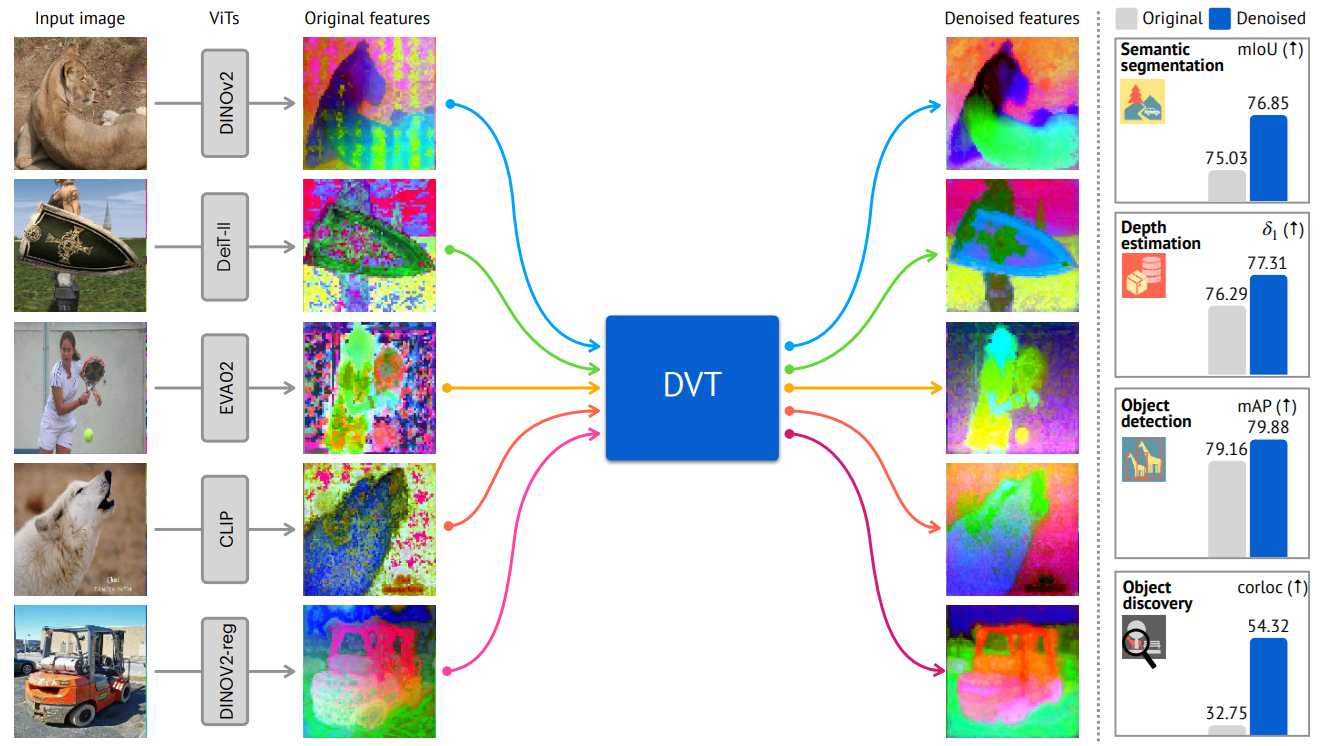
\includegraphics[width=0.5\textwidth]{figures/artifacts-positions.png}
  %   \caption{Demonstration of \ac{dvt}. Image obtained from \cite{denoising}}
  %   \label{fig:artifacts-positions}
  % \end{figure}

  \section{Conclusion}
  The conclusion goes here.

  \printbibliography

  \begin{acronym}
    \acro{vit}[ViT]{Vision Transformer}
    \acro{nlp}[NLP]{Natural Language Processing}
    \acro{cnn}[CNN]{Convolutional Neural Network}
    \acroplural{cnn}[CNNs]{\acp{cnn}}
    \acro{rnn}[RNN]{Recurrent Neural Network}
    \acro{mlp}[MLP]{Multi-Layer Perceptron}
    \acro{ssm}[SSM]{State Space Model}
    \acro{clip}[CLIP]{Contrastive Language-Image Pre-training}
    \acro{dvt}[DVT]{Denoising Vision Transformers}
  \end{acronym}


that's all folks
\end{document}


